\documentclass[14pt]{extbook}
\usepackage{multicol, enumerate, enumitem, hyperref, color, soul, setspace, parskip, fancyhdr} %General Packages
\usepackage{amssymb, amsthm, amsmath, latexsym, units, mathtools} %Math Packages
\everymath{\displaystyle} %All math in Display Style
% Packages with additional options
\usepackage[headsep=0.5cm,headheight=12pt, left=1 in,right= 1 in,top= 1 in,bottom= 1 in]{geometry}
\usepackage[usenames,dvipsnames]{xcolor}
\usepackage{dashrule}  % Package to use the command below to create lines between items
\newcommand{\litem}[1]{\item#1\hspace*{-1cm}\rule{\textwidth}{0.4pt}}
\pagestyle{fancy}
\lhead{Progress Quiz 6}
\chead{}
\rhead{Version A}
\lfoot{9689-6866}
\cfoot{}
\rfoot{Spring 2021}
\begin{document}

\begin{enumerate}
\litem{
Graph the equation below.\[ f(x) = -(x-3)^2 + 17 \]\begin{enumerate}[label=\Alph*.]
\begin{multicols}{2}\item 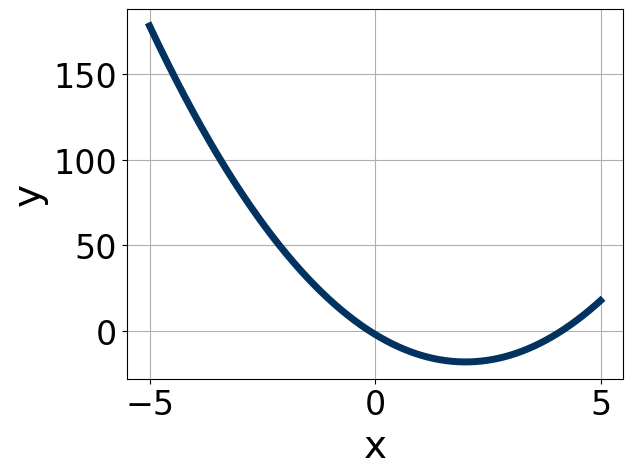
\includegraphics[width = 0.3\textwidth]{../Figures/quadraticEquationToGraphAA.png}\item 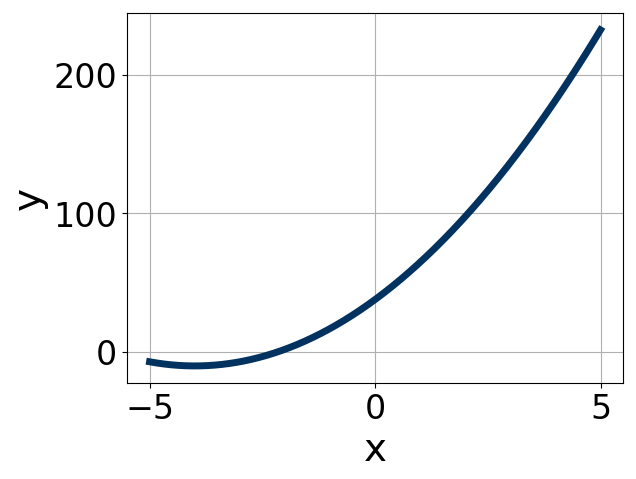
\includegraphics[width = 0.3\textwidth]{../Figures/quadraticEquationToGraphBA.png}\item 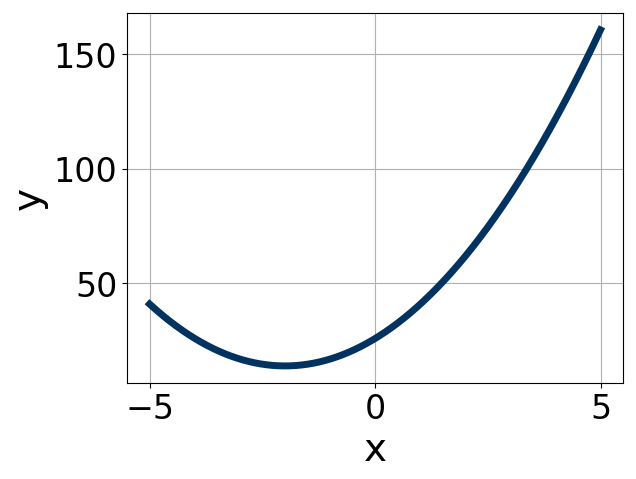
\includegraphics[width = 0.3\textwidth]{../Figures/quadraticEquationToGraphCA.png}\item 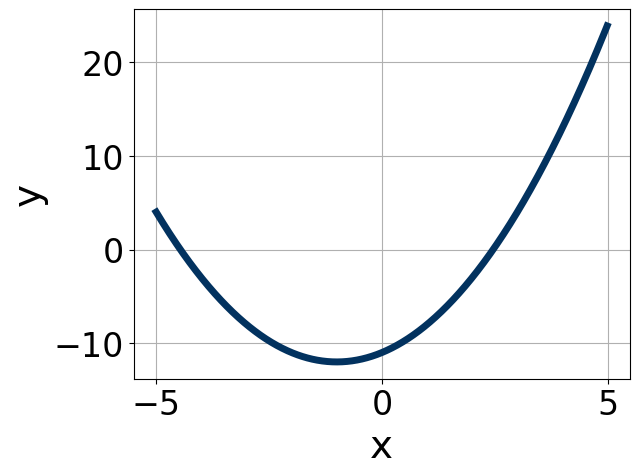
\includegraphics[width = 0.3\textwidth]{../Figures/quadraticEquationToGraphDA.png}\end{multicols}\item None of the above.
\end{enumerate} }
\litem{
Solve the quadratic equation below. Then, choose the intervals that the solutions belong to, with $x_1 \leq x_2$ (if they exist).\[ 17x^{2} -15 x -9 = 0 \]\begin{enumerate}[label=\Alph*.]
\item \( x_1 \in [-29.5, -28] \text{ and } x_2 \in [28.4, 29.7] \)
\item \( x_1 \in [-8, -6.7] \text{ and } x_2 \in [20.5, 23.2] \)
\item \( x_1 \in [-2.6, -0.9] \text{ and } x_2 \in [0.2, 1.1] \)
\item \( x_1 \in [-0.5, 0.4] \text{ and } x_2 \in [1.2, 2.9] \)
\item \( \text{There are no Real solutions.} \)

\end{enumerate} }
\litem{
Solve the quadratic equation below. Then, choose the intervals that the solutions $x_1$ and $x_2$ belong to, with $x_1 \leq x_2$.\[ 15x^{2} -2 x -24 = 0 \]\begin{enumerate}[label=\Alph*.]
\item \( x_1 \in [-6.12, -5.71] \text{ and } x_2 \in [-0.1, 0.4] \)
\item \( x_1 \in [-18.29, -17.87] \text{ and } x_2 \in [19.9, 20.05] \)
\item \( x_1 \in [-2.42, -2.16] \text{ and } x_2 \in [0.47, 0.98] \)
\item \( x_1 \in [-1.13, -0.44] \text{ and } x_2 \in [2.6, 3.13] \)
\item \( x_1 \in [-1.34, -1.07] \text{ and } x_2 \in [1.16, 1.37] \)

\end{enumerate} }
\litem{
Write the equation of the graph presented below in the form $f(x)=ax^2+bx+c$, assuming  $a=1$ or $a=-1$. Then, choose the intervals that $a, b,$ and $c$ belong to.
\begin{center}
    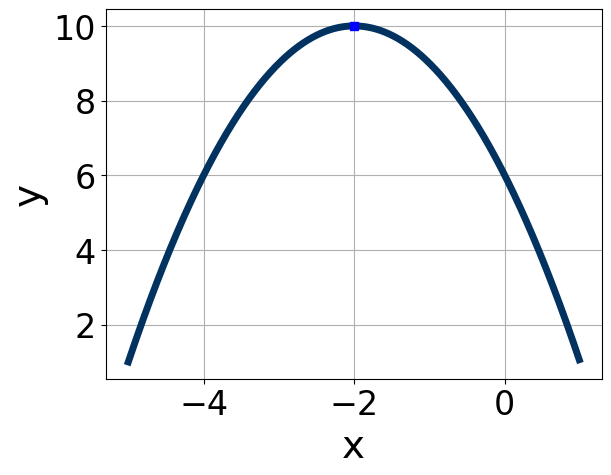
\includegraphics[width=0.5\textwidth]{../Figures/quadraticGraphToEquationCopyA.png}
\end{center}
\begin{enumerate}[label=\Alph*.]
\item \( a \in [-1.1, -0.3], \hspace*{5mm} b \in [-9, -4], \text{ and } \hspace*{5mm} c \in [-24, -20] \)
\item \( a \in [0, 2.4], \hspace*{5mm} b \in [-9, -4], \text{ and } \hspace*{5mm} c \in [7, 9] \)
\item \( a \in [-1.1, -0.3], \hspace*{5mm} b \in [-9, -4], \text{ and } \hspace*{5mm} c \in [-9, -6] \)
\item \( a \in [0, 2.4], \hspace*{5mm} b \in [8, 10], \text{ and } \hspace*{5mm} c \in [7, 9] \)
\item \( a \in [-1.1, -0.3], \hspace*{5mm} b \in [8, 10], \text{ and } \hspace*{5mm} c \in [-24, -20] \)

\end{enumerate} }
\litem{
Factor the quadratic below. Then, choose the intervals that contain the constants in the form $(ax+b)(cx+d); b \leq d.$\[ 36x^{2} -60 x + 25 \]\begin{enumerate}[label=\Alph*.]
\item \( a \in [2.3, 5.3], \hspace*{5mm} b \in [-5, -4], \hspace*{5mm} c \in [10, 12.4], \text{ and } \hspace*{5mm} d \in [-9, -4] \)
\item \( a \in [3.4, 6.6], \hspace*{5mm} b \in [-5, -4], \hspace*{5mm} c \in [5.2, 9.8], \text{ and } \hspace*{5mm} d \in [-9, -4] \)
\item \( a \in [11.7, 13.1], \hspace*{5mm} b \in [-5, -4], \hspace*{5mm} c \in [1.9, 4.1], \text{ and } \hspace*{5mm} d \in [-9, -4] \)
\item \( a \in [-0.6, 1.1], \hspace*{5mm} b \in [-34, -27], \hspace*{5mm} c \in [-0.8, 1.4], \text{ and } \hspace*{5mm} d \in [-35, -27] \)
\item \( \text{None of the above.} \)

\end{enumerate} }
\litem{
Write the equation of the graph presented below in the form $f(x)=ax^2+bx+c$, assuming  $a=1$ or $a=-1$. Then, choose the intervals that $a, b,$ and $c$ belong to.
\begin{center}
    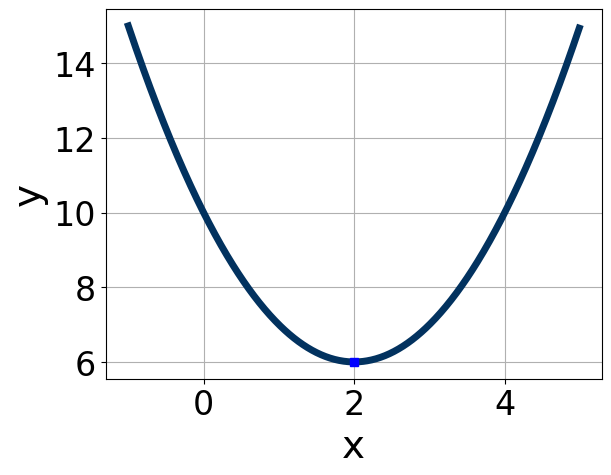
\includegraphics[width=0.5\textwidth]{../Figures/quadraticGraphToEquationA.png}
\end{center}
\begin{enumerate}[label=\Alph*.]
\item \( a \in [0, 4], \hspace*{5mm} b \in [2, 7], \text{ and } \hspace*{5mm} c \in [-6, -5] \)
\item \( a \in [0, 4], \hspace*{5mm} b \in [-4, -1], \text{ and } \hspace*{5mm} c \in [-6, -5] \)
\item \( a \in [-4, 0], \hspace*{5mm} b \in [2, 7], \text{ and } \hspace*{5mm} c \in [5, 8] \)
\item \( a \in [-4, 0], \hspace*{5mm} b \in [-4, -1], \text{ and } \hspace*{5mm} c \in [-14, -10] \)
\item \( a \in [-4, 0], \hspace*{5mm} b \in [2, 7], \text{ and } \hspace*{5mm} c \in [-14, -10] \)

\end{enumerate} }
\litem{
Solve the quadratic equation below. Then, choose the intervals that the solutions $x_1$ and $x_2$ belong to, with $x_1 \leq x_2$.\[ 25x^{2} +50 x + 24 = 0 \]\begin{enumerate}[label=\Alph*.]
\item \( x_1 \in [-1.52, -0.85] \text{ and } x_2 \in [-1.12, -0.8] \)
\item \( x_1 \in [-1.78, -1.45] \text{ and } x_2 \in [-0.68, -0.53] \)
\item \( x_1 \in [-2.75, -2.1] \text{ and } x_2 \in [-0.42, -0.26] \)
\item \( x_1 \in [-30.38, -29.84] \text{ and } x_2 \in [-20.28, -19.95] \)
\item \( x_1 \in [-6.22, -5.97] \text{ and } x_2 \in [-0.26, -0.15] \)

\end{enumerate} }
\litem{
Factor the quadratic below. Then, choose the intervals that contain the constants in the form $(ax+b)(cx+d); b \leq d.$\[ 24x^{2} +2 x -15 \]\begin{enumerate}[label=\Alph*.]
\item \( a \in [2.78, 4.57], \hspace*{5mm} b \in [-3, -1], \hspace*{5mm} c \in [4.7, 11.7], \text{ and } \hspace*{5mm} d \in [0, 8] \)
\item \( a \in [0.86, 1.33], \hspace*{5mm} b \in [-19, -16], \hspace*{5mm} c \in [-0.5, 1.9], \text{ and } \hspace*{5mm} d \in [17, 27] \)
\item \( a \in [1.02, 2.41], \hspace*{5mm} b \in [-3, -1], \hspace*{5mm} c \in [9.4, 16.1], \text{ and } \hspace*{5mm} d \in [0, 8] \)
\item \( a \in [11.87, 13.85], \hspace*{5mm} b \in [-3, -1], \hspace*{5mm} c \in [1.7, 3.4], \text{ and } \hspace*{5mm} d \in [0, 8] \)
\item \( \text{None of the above.} \)

\end{enumerate} }
\litem{
Solve the quadratic equation below. Then, choose the intervals that the solutions belong to, with $x_1 \leq x_2$ (if they exist).\[ 19x^{2} -9 x -2 = 0 \]\begin{enumerate}[label=\Alph*.]
\item \( x_1 \in [-0.48, 0.13] \text{ and } x_2 \in [0.51, 0.67] \)
\item \( x_1 \in [-3.37, -3] \text{ and } x_2 \in [11.25, 12.8] \)
\item \( x_1 \in [-1.04, -0.42] \text{ and } x_2 \in [-0.24, 0.26] \)
\item \( x_1 \in [-15.25, -14.96] \text{ and } x_2 \in [15.15, 16.25] \)
\item \( \text{There are no Real solutions.} \)

\end{enumerate} }
\litem{
Graph the equation below.\[ f(x) = (x+1)^2 - 20 \]\begin{enumerate}[label=\Alph*.]
\begin{multicols}{2}\item 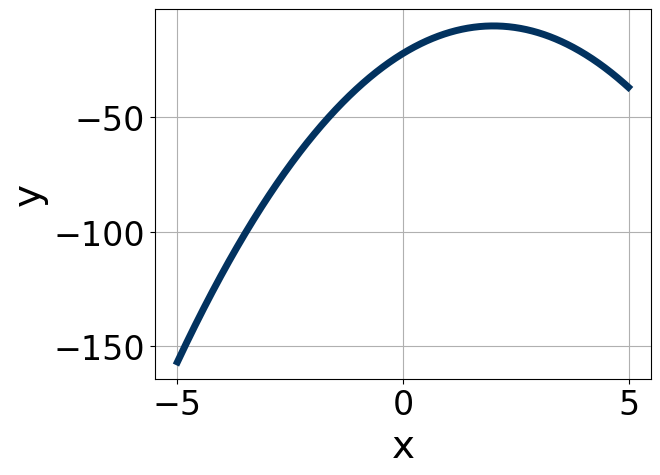
\includegraphics[width = 0.3\textwidth]{../Figures/quadraticEquationToGraphCopyAA.png}\item 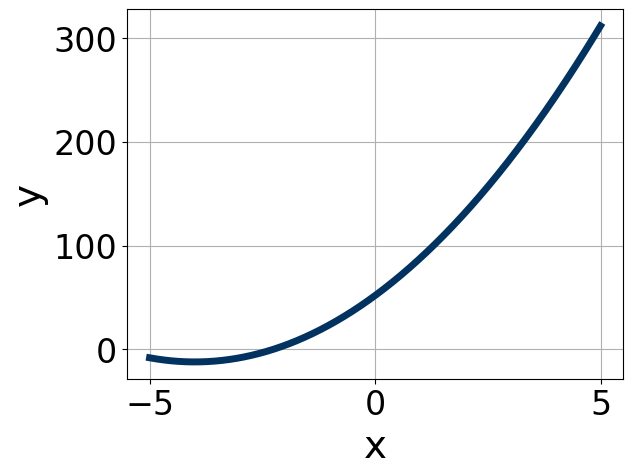
\includegraphics[width = 0.3\textwidth]{../Figures/quadraticEquationToGraphCopyBA.png}\item 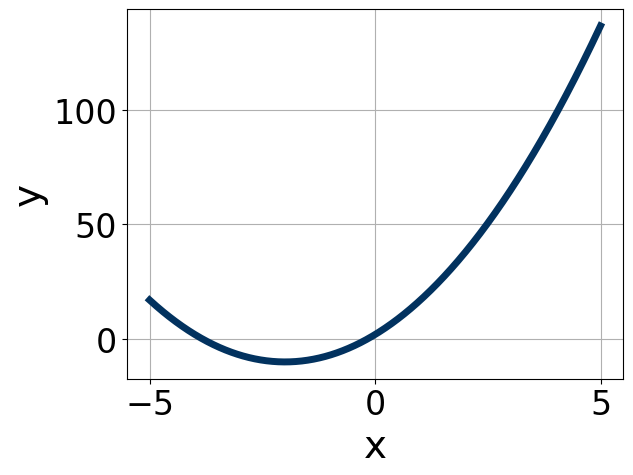
\includegraphics[width = 0.3\textwidth]{../Figures/quadraticEquationToGraphCopyCA.png}\item 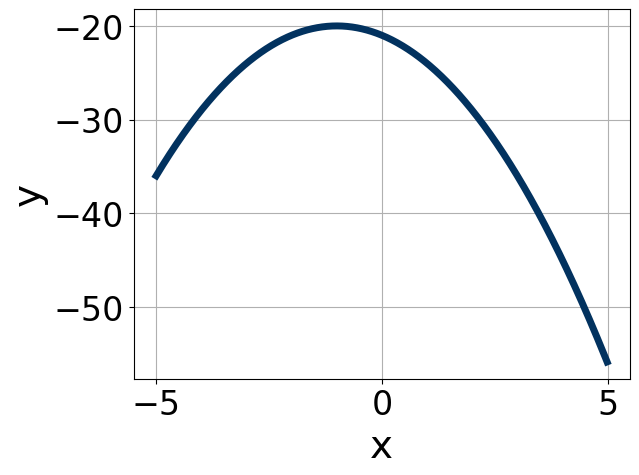
\includegraphics[width = 0.3\textwidth]{../Figures/quadraticEquationToGraphCopyDA.png}\end{multicols}\item None of the above.
\end{enumerate} }
\end{enumerate}

\end{document}